\subsection{TP : Un exemple complet dans un cadre de fiabilité industrielle }

Soit $X$ la durée de vie d'un composant $\Sigma$, supposé tomber uniquement en panne par hasard. Le taux de défaillance $\lambda$ de $\Sigma$ est donc constant, ce qui implique  $X\sim {\cal{E}}(\lambda)$. Il est courant de disposer d'un  expert industriel  familier de $\lambda$, avec qui le dialogue suivant peut être engagé. 
 "Considérons une décision de management (remplacement) établie sur une valeur donnée $\bar{\lambda}$ \emph{(différente de la vraie valeur inconnue $\lambda$)}
\item Pour un \emph{co\^ut} similaire  $|\bar{\lambda}-\lambda|$, il y a 2 conséquences possibles au remplacement : 
\begin{itemize}
\item  soit $C_1$ le co\^ut positif moyen d'\^etre trop optimiste (d'avoir $\bar{\lambda}\leq \lambda$) ; 
\item  soit $C_2$ le co\^ut positif moyen d'\^etre trop pessimiste (d'avoir $\bar{\lambda}>\lambda$). 
\item Pouvez-vous donner un estimé $\hat{\delta}$ du rapport des co\^uts moyens $\delta=C_2/C_1$" ?
\end{itemize}
L'axiome de rationalité dit que si l'expert n'est pas \emph{averse au risque}, alors 
\begin{eqnarray*}
\bar{\lambda} & = & \arg\min_{x} \underbrace{\int_{0}^{\infty} \left|x-\lambda\right|\left(C_1\1_{\{x\leq \lambda\}} + C_2\1_{\{x>\lambda\}}\right) \pi(\lambda) \ d\lambda}_{\text{\tiny fonction de co\^ut intégr\'ee sur toutes les valeurs possibles {\it a priori} du vrai $\lambda$}} 
\end{eqnarray*}
\begin{eqnarray*}
\text{ Il s'ensuit que} \ \ \ \ \int_{0}^{\bar{\lambda}} d\Pi(\lambda) & = & \Pi(\lambda<\bar{\lambda}) \ = \ \frac{C_1}{C_1+C_2}.  
\end{eqnarray*} 
 L'interprétation de la réponse de l'expert est que $1/(1+\hat{\delta})$ est un estimé du quantile {\it a priori} d'ordre $\alpha=C_1/(C_1+C_2)$. 
Avec $P(\lambda<\bar{\lambda})=\frac{C_1}{C_1+C_2}=\alpha$, on a :
\begin{itemize}
\item tant que les co\^uts sont équilibrés, un expert de plus en plus optimiste fournira un $\bar{\lambda}$ de plus en plus petit, car la durée moyenne avant la prochaine défaillance est
\begin{eqnarray*}
\E[X|\lambda] & = &  \frac{1}{\lambda}.
\end{eqnarray*}
 
\item cependant l'expert s'exprime plutôt sur les co\^uts lorsqu'on lui fournit une valeur représentative de $\bar{\lambda}$ : 
\begin{itemize} 
\item   plus l'expert est optimiste, plus le co\^ut $C_2$ d'\^etre optimiste (selon lui) est petit, donc $\alpha$ grandit vers 1 et
\begin{eqnarray*}
\E[X] & = & \E[\E[X|\lambda]] \ = \ \E[1/\lambda] \ \ \text{augmente}.
\end{eqnarray*}
\item   plus l'expert est pessimiste, plus le co\^ut $C_2$ d'\^etre optimiste augmente, donc $\alpha$ tombe vers 0 et
\begin{eqnarray*}
\E[X] & = &  \E[1/\lambda] \ \ \text{diminue}.
\end{eqnarray*}
\end{itemize}
\end{itemize} 
Quelle choix de loi {\it a priori} pouvons-nous proposer au décideur ?



\if\mycmdtpthree1 \paragraph{\bf Réponse.} \\

On raisonne par \emph{données virtuelles} : 
\begin{itemize}
\item L'{\it a priori} non-informatif de Jeffreys est utilisé pour modéliser l'absence d'expertise et la simple connaissance du modèle 
\begin{eqnarray*}
\pi_{0}(\lambda) & \propto \lambda^{-1}  \ \ \ \ \ \ \ \ \text{ {\it (paramètre d'échelle)}}. 
\end{eqnarray*} 
\item L'information apportée par l'expert est assimilée à celle apportée par un échantillon i.i.d. 
\begin{eqnarray*}
{\bf x_m} & \sim & {\cal{E}}(\lambda).
\end{eqnarray*}
\item Un ``bon" prior informatif pour $\lambda$ est donc $\pi(\lambda)=\pi_0(\lambda|{\bf x_m})$, soit
\begin{eqnarray*}
\lambda & \sim & {\cal{G}}(m,m \bar{\bf x}_m).
\end{eqnarray*} 
\end{itemize}
Donc $2m \bar{\bf x}_m \lambda \sim {\cal{G}}(m,1/2) \equiv \chi^2_{2m}$, d'où ${\displaystyle \bar{\bf x}_m  =  \frac{\chi^2_{2m}(\alpha)}{2m\bar{\lambda}}}$. Le décideur peut fixer arbitraitement $m$ selon la confiance qu'il a en l'expert {(ou mettre un {\it a priori} hiérarchique dessus)}. De plus, l'{\it a priori} est \emph{conjugué} : sachant des durées de vie observées ${\bf x_n}=(x_1,\ldots,x_n)$, la loi {\it a posteriori} de $\lambda$ est
\begin{eqnarray*}
\lambda|{\bf x_n} & \sim & {\cal{G}}\left(m+n,\frac{\chi^2_{2m}(\alpha)}{2\bar{\lambda}} + n\sum\limits_{i=1}^n x_i\right)
\end{eqnarray*} 
L'ingénieur s'intéresse alors à la probabilité \emph{prédictive} que $\Sigma$ tombe en panne avant la prochaine visite au temps $x_0$
\begin{eqnarray*}
P\left(X<x_0\right)  & = & \int_{0}^{\infty} P\left(X<x_0|\lambda\right) \pi(\lambda|{\bf x_n}) \ d\lambda \ = \ 
                   1 - 1/\left(1 + \frac{x_0}{\frac{\chi^2_{2m}(\alpha)}{2\bar{\lambda}} + n\sum\limits_{i=1}^n x_i}\right)^{m+n}
\end{eqnarray*}
puis il peut introduire une fonction de co\^ut, etc. pour prendre une décision. Les figures suivantes (\ref{expert1} à \ref{expert3}) illustrent ainsi différents comportements {\it a posteriori}, lorsqu'on simule 10 données selon ${\cal{E}}(\lambda_0)$ avec $\lambda_0=1/10$. \\ 

\begin{figure}[h!]
\centering
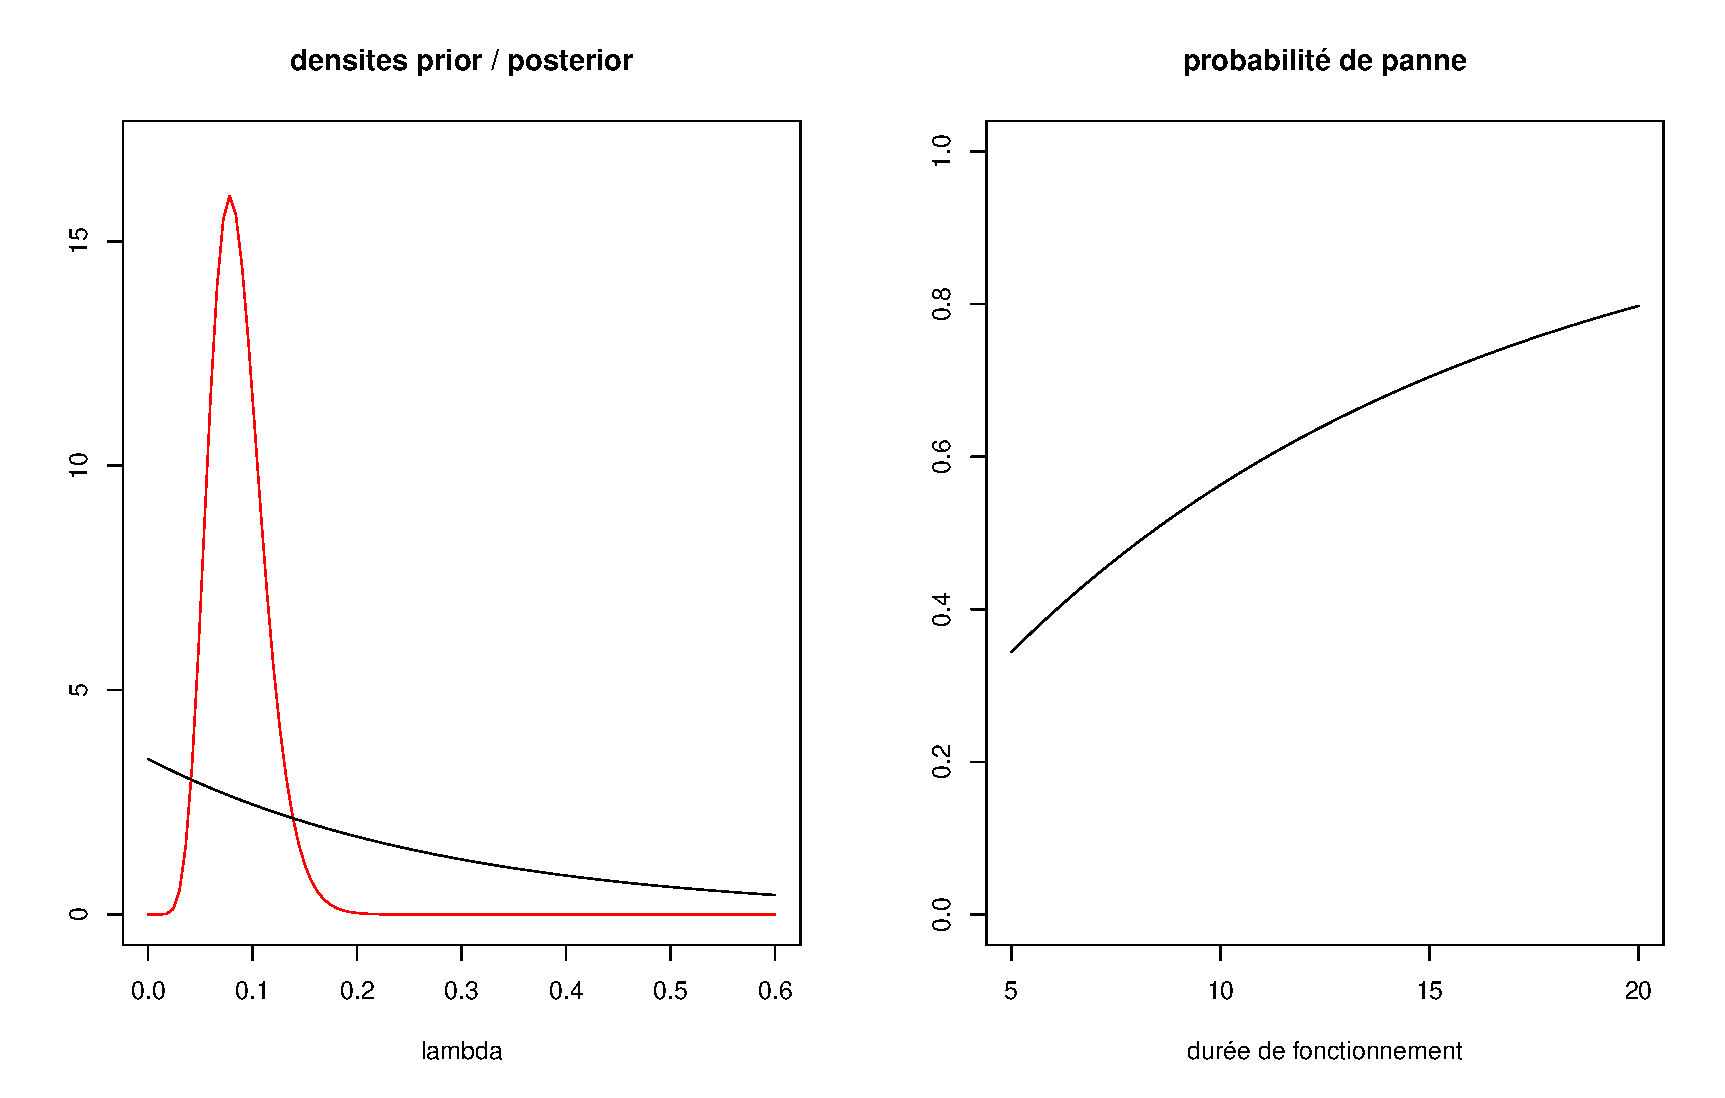
\includegraphics[scale=0.4]{figures/prior/figure01.pdf} 
\caption{$m=1$, $\bar{\lambda}=1/5$, $\alpha=50\%$ (expert peu informatif et pessimiste).}
\label{expert1}
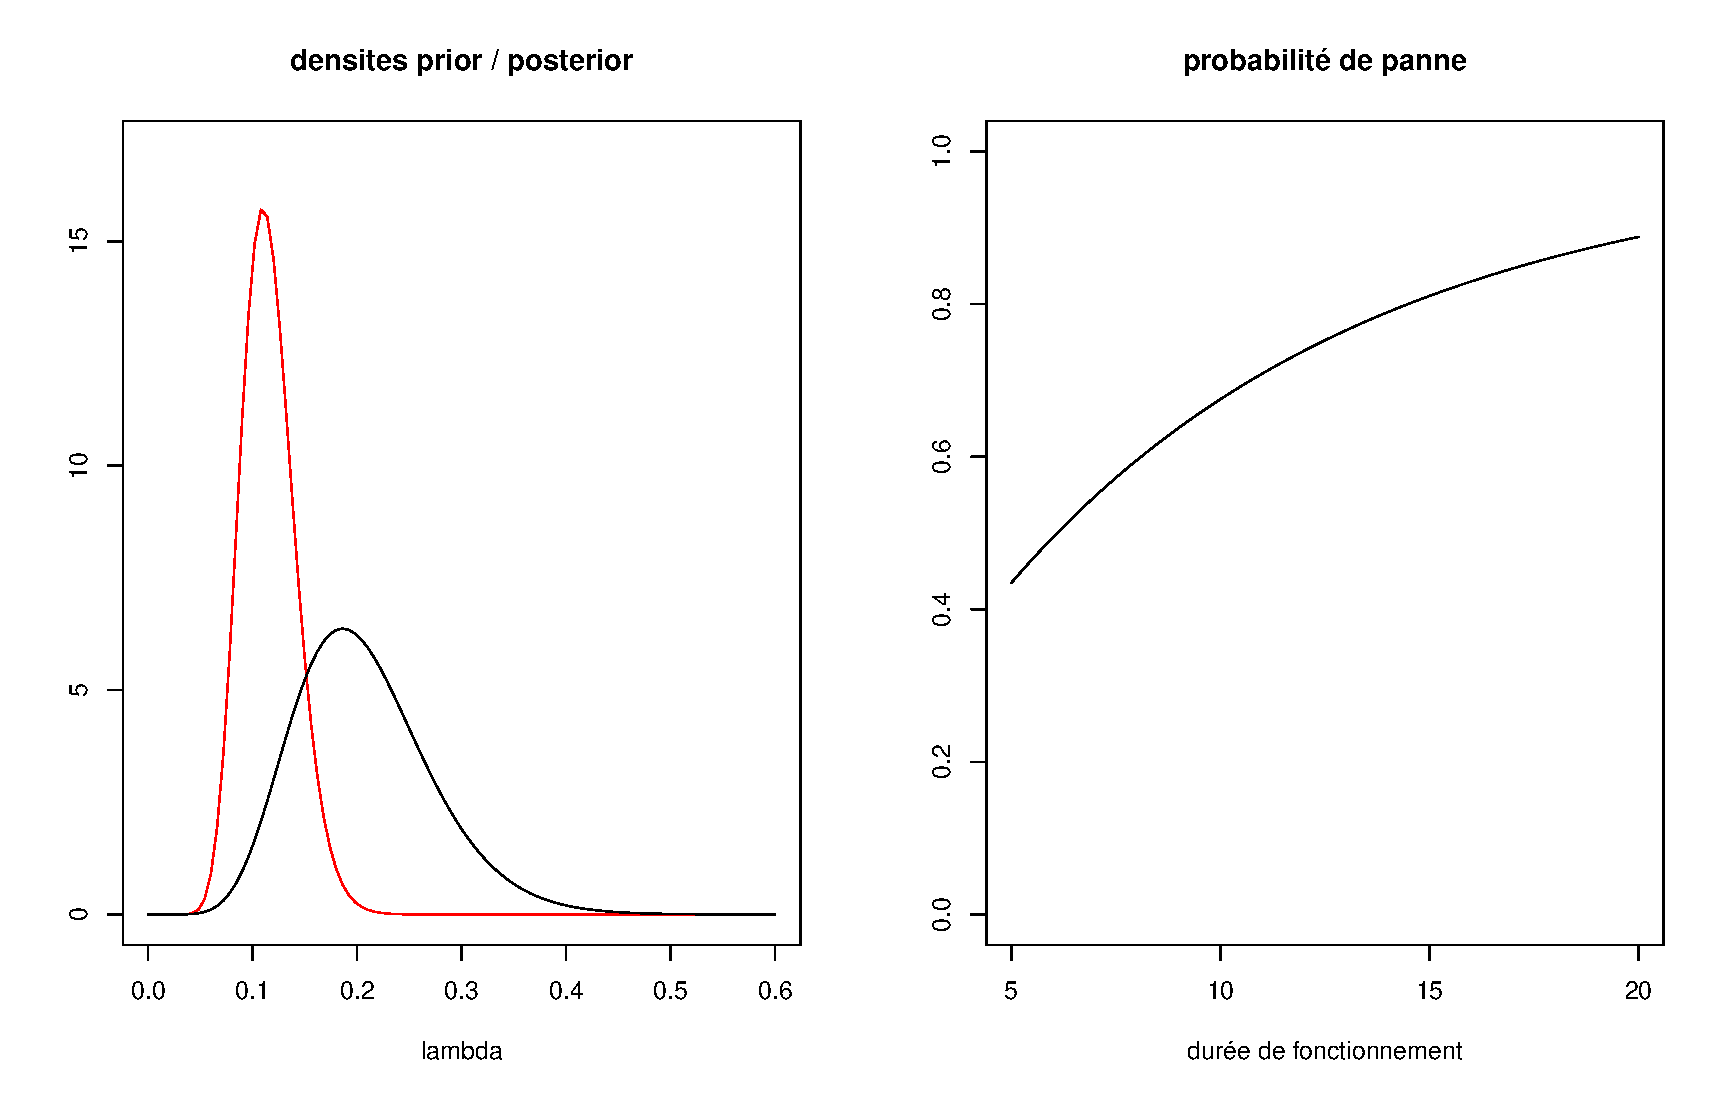
\includegraphics[scale=0.4]{figures/prior/figure02.pdf} 
\caption{$m=10$, $\bar{\lambda}=1/5$, $\alpha=50\%$ (expert très informatif et pessimiste).} \label{expert2}
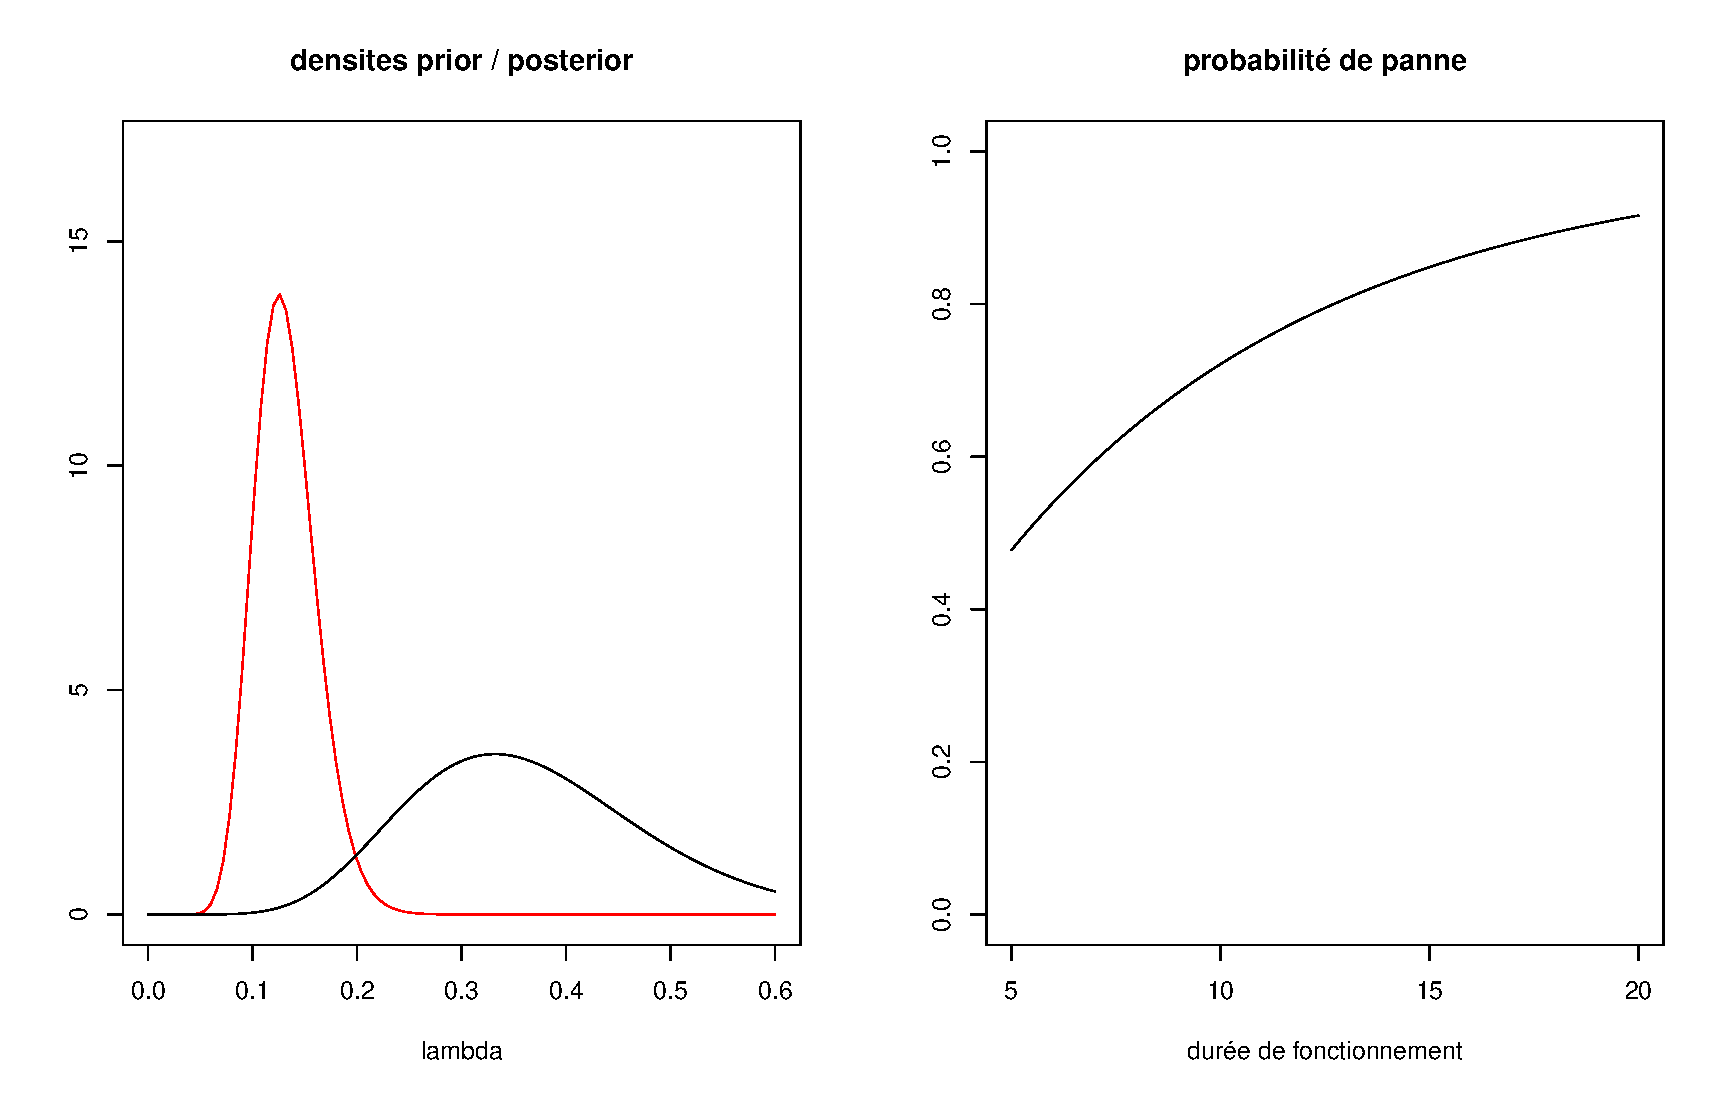
\includegraphics[scale=0.4]{figures/prior/figure03.pdf} 
\caption{$m=10$, $\bar{\lambda}=1/5$, $\alpha=5\%$ (expert très informatif et très pessimiste).} \label{expert3}
\end{figure}

En fait, plus habituellement, l'expert préfère exprimer son opinion \emph{quantitative} sur la durée de vie $X$
 ($=$ \emph{variable d'ancrage}) que sur $\lambda$, car $X$ est {\bf observable}. Dans ce cas, il est assimilé à un fournisseur d'estimé du \emph{quantile prédictif {\it a priori}} $\bar{x}$ :
\begin{eqnarray*}
\int_{0}^{\bar{x}} f(x) \ dx & = & \int_{0}^{\bar{x}} \int_{\Theta} f(x|\theta)\pi(\theta) \ d\theta \ = \ \alpha
\end{eqnarray*}
Cette interprétation est la plus acceptée en général dans la communauté statistique bayésienne, c'est pourquoi les statisticiens fiabilistes préfèrent poser des questions comme : 
\begin{eqnarray*}
\text{\it Sachant les temps $x_0$ et $x_1>x_0$, $\Sigma$ a $1-\alpha$ fois plus de chance de ne pas tomber en panne après $x_0$ qu'après $x_1$.} \\
\text{\it Quelle est votre évaluation de $1-\alpha$ ?} 
\end{eqnarray*}
%\item La réponse est un estimé de $\P(X>x_0)/P(X>x_1)$

\fi